
%-----------------------------------------------------
%
%    Contents
%
%-----------------------------------------------------

\sectionfix
\section{Design Goals}
\label{sec:goals}
This chapter describes the goal of our design tool and briefly outlines the design considerations. Additionally, we present an architectural pipeline on how we achieved this task. 
\subsection{Requirements}
Advances in research have shown that worn electronics and sensors can enable the human body to be more interactive in context of how we complete daily and complex tasks in an efficient way \cite{Amft:2008:RDA:1343127.1343441}. While the technology constantly evolves around optimizing and building novel sensors, there are still challenges to be considered in regards to the fabrication process and its resulting costs. Our idea is to put upon the research domain of computer graphics and human-computer interaction to ease the aforementioned process by providing the user a graphical interface for designing their own on-body sensors. The tool is required to be guiding the user through its main functionality, provide fast iterable setup and be able to support multiple body locations and users. Our software prototype pursues these six following requirements.
\raggedbottom
\paragraph*{Rapid Prototyping}
\begin{description}
\item[R1] Allow the user to apply design ideas quickly within the system
\item[R2] Provide a fast iterative workflow
\item[R3] Maintain an easy to use interface
\item[R4] Offer a system that can be set-up effortlessly
\end{description}

\paragraph*{Flexible Scalability \& Design}  
\begin{description}
\item[R5] Must be applicable to multiple locations on the arm
\item[R6] Must be applicable to all users \\[3.25ex]
\end{description}

While the design and fabrication process of sensors is rather common nowadays, it raises a number of challenges to people that do not have the required technical background to produce sensors for their own uses. The design tool is therefore inclined to fit users that do not have that expertise but want to have their own sensor design fabricated rapidely. This aspect is summarized in \textbf{R1}. When asked to design specific images, many people are not confident in their own skills and will hence be hesitant about it \cite{Dixon:2010:IUS:1753326.1753459}. Therefore, many drawing softwares offer the flexibility to import existing templates into the tool \cite{Iarussi:2013:DAA:2501988.2501997, Fernquist:2011:SRE:2047196.2047245}. This creates an initial starting point for the users and helps them to be more creative with their own work which leads to our second requirement \textbf{R2}. On the other hand, \textbf{R3} is based on the consensus that an intuitive interface also directly accelerate the work flow of the process itself and improves the user experience \cite{Hassenzahl:2008:UET:1512714.1512717}. This criteria is a must-have for any interfaces targeting users without advanced knowledge of such tools.\\ Camera-based systems are often used in research domain to model environments in real dimensions, track movements or identify objects. However, there are a lot of products that are expensive since they are dependant on several cameras, large areas, certain lighting conditions or multiple people to set up \cite{Rahimian:2015:OCP:2821592.2821596, Dezfuli:2012:PIP:2325616.2325623}. \textbf{R4} targets these problems for users that do not have the resources mentioned above.\\Regarding the scalability, the core idea behind \textbf{R5} is to provide the user a feeling of intimate customization during the design process \cite{Kao:2016:DRP:2971763.2971777} while \textbf{R6} focuses on the fact that anyone should be able to use the software regardless of their unique body size \cite{Nittala:2018:MST:3173574.3173607, Dezfuli:2012:PIP:2325616.2325623}.\newpara
In this section, we have presented a list of requirements which aligns with our vision of a personalized fabrication process for on-body sensors. Following, we will discuss the demanding challenges and open research questions that existed during our work and realization of the previously mentioned points.
\subsection{Challenges}
We came across multiple technical difficulties during our research on how we wanted to achieve this goal. 
\paragraph*{Digital Model Acquisition} The human anatomy is a widespread topic. 
Each human's body is as unique as one's own fingerprint. Properties such as skin color, skin elasticity, size and irregularities on the body define our individual characteristics \cite{Nittala:2018:MST:3173574.3173607}. Capturing all of those unique attributes is a prominent research challenge in computer vision. A solution to this problem is the use of a camera-based scanning and reconstruction method which is able to leverage most of these properties. This approach is ideal for complex geometries that require a massive amount of data for an accurate description of its surface \cite{Gopi:2002:FEP:646016.678279}. The acquisition initially creates point clouds of data from the outer form of the object. Afterwards, the resulting information allows us to digitally capture the exact size and shape of the physical object into the computer as a digital 3-dimensional ( 3D ) representation e.g. a body part in virtual environment. At last, post-processing methods are applied to the dataset which can include fixing holes, filtering noises or classification \cite{Weyrich:2004:PSS:2386332.2386347} to finalize the reconstruction.\\
A number of digital models of body parts can also be acquired by capturing mid-air gestures and a search through populated databases \cite{Holz:2011:DMI:1978942.1979060}. However, these geometries vary massively in their resolutions and will therefore not provide an idealized model for personalized design.
\newpara
As previously mentioned in the related work, we will focus on the reconstruction of the human arm as it offers the most comfortable surface for touch input and gives the best haptic feedback to the users \cite{Harrison:2014:ILT:2598510.2598587, Weigel:2014:MTU:2556288.2557239}. Remarkably, hands were also highly rated among the study participants but because of its joints and complex non-flat surface it was rather hard to interact with. The form of the forearm was more straight forward and aligned to a flat touchpad commonly known in laptops.
\paragraph*{Camera Parametrization}
A 3D scan can either be a result of a simple RGB-D camera \cite{Wilson:2010:UDC:1936652.1936665, Dezfuli:2012:PIP:2325616.2325623} or a complex motion-capture technology \cite{Gannon:2016:EOF:2858036.2858576}. Both setups have their own benefits and drawbacks. The RGB-D camera is reliant on a more software-oriented process to retrieve the depth information of the device and to reconstruct a 3d model. Depending on the cost of the software, this approach can be very cost efficient and fast to set up. On the other hand, a mocap system is rather expensive nowadays since it uses a lot of cameras to capture different angles. Furthermore, it is usually restricted to a certain room space which might not always be available. However, the results can be worth the time and money since it provides a more realistic image of the scenery which is important for particular application domains e.g. animations in movies.\newpara
In our case, we decided to use the motion-sensing device Kinect (2nd generation) which is produced by Microsoft. Kinect contains an RGB camera, a depth sensor, an IR emitter and a multi-array microphone (see \textbf{\autoref{fig:kinect}}).\newpara
\begin{figure}[H]
    \centering
    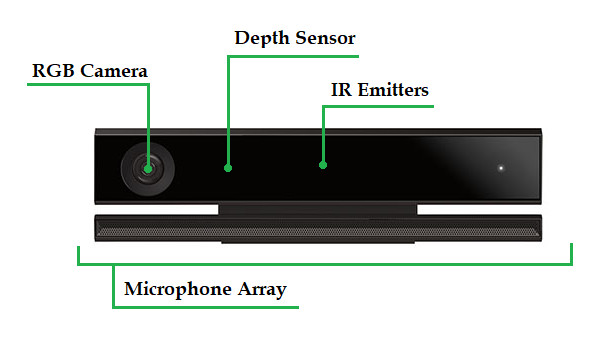
\includegraphics[scale=0.7]{pictures/kinect.png}
    \caption{Architecture of 2nd generation Kinect}
    \label{fig:kinect}
\end{figure}
By emitting light signals and then measuring how long it takes them to return, Kinect is able to differentiate light reflecting from objects in a room and therefore provide an accurate depth estimation. This technology is referred to as the \textit{time-of-flight} ( TOF ) method \cite{lachat2015first, sell2014xbox}. Due to its affordable price compared to most of the 3D scanners on the market, many researchers and private consumers are using the Kinect as a tool for tracking the human body \cite{Harrison:2011:OWM:2047196.2047255, Dezfuli:2012:PIP:2325616.2325623, Wilson:2010:UDC:1936652.1936665}. Additionally, the second version of its product line obtains much better resolution while also reducing noises and interferences from outside IR sources \cite{wasenmuller2016comparison}.\\
With the capability of its SDK, we are able to use the Kinect as a low-cost handheld sensor to scan different parts of an object and work with its resulting organized point clouds.

\paragraph*{Design Environment}
As previously mentioned in the related work, digital design tool has been developed for various hybrid applications in fabrication. Most of the work has been focusing on using the skin as an interactive surface for gestural or machine input. These digital fabrication approaches enable non-experts to intuitively create precise shapes on top of complex physical surroundings. While these technologies open up a large design space for users without the technical background to the fabrication process, there is not yet a pipeline that connects the design process with a higher level user interface. This approach gives the user more flexibility in their creative customization process and yields a good balance between rapid prototyping and sophisticated design on a representational model.\\
Using a digital process also enables us to translate existing analog methods into a more computational workflow. Manipulating patterns like scaling, positioning, duplicating and reorienting is a time-consuming task in the real world but is easily integrated into our tool. Sharing your own designs with multiple users is another benefit. It enables others to review your work and contribute to it which in return improves the product. Furthermore, design process often happens simultaneously with a lot of different iterations before committing to an end result. The capability to visualize a current prototype vastly improves the design-to-production workflow and can offer a much broader control over the final outcome. At last, a user interface provides a natural mean to guide the user and give him feedback on its current iteration. This user-centric approach helps every user to build their own sensors without consuming too much time on the process itself. In combination with the Kinect, the design environment offers an initial easy-to-setup and cheap approach for customized sensor designs.

\subsection{Overview}
\label{subsec:overview}
The goal of this work is to allow the user to create a flatten 3D shape of a body part for personalized on-body sensors using the RGB-D camera Kinect and our design tool. Therewith, the rigid volumetric representation of an arm is reconstructed and further processed for display to the user. Unlike to related work, this approach highly focuses on the precise geometry acquisition of the scanned object and on the flexibility of the tool for rapid prototyping. A pipeline overview of the sequential steps performed for each depth frame is depicted in \textbf{\autoref{fig:pipeline}}. Some of the algorithms listed in this part are tailored to the existing approaches of KinectFusion \cite{Izadi:2011:KRR:2047196.2047270} which will be discussed profoundly in \autoref{sec:implementation}.\newpara

\begin{figure}[ht]
    \centering
  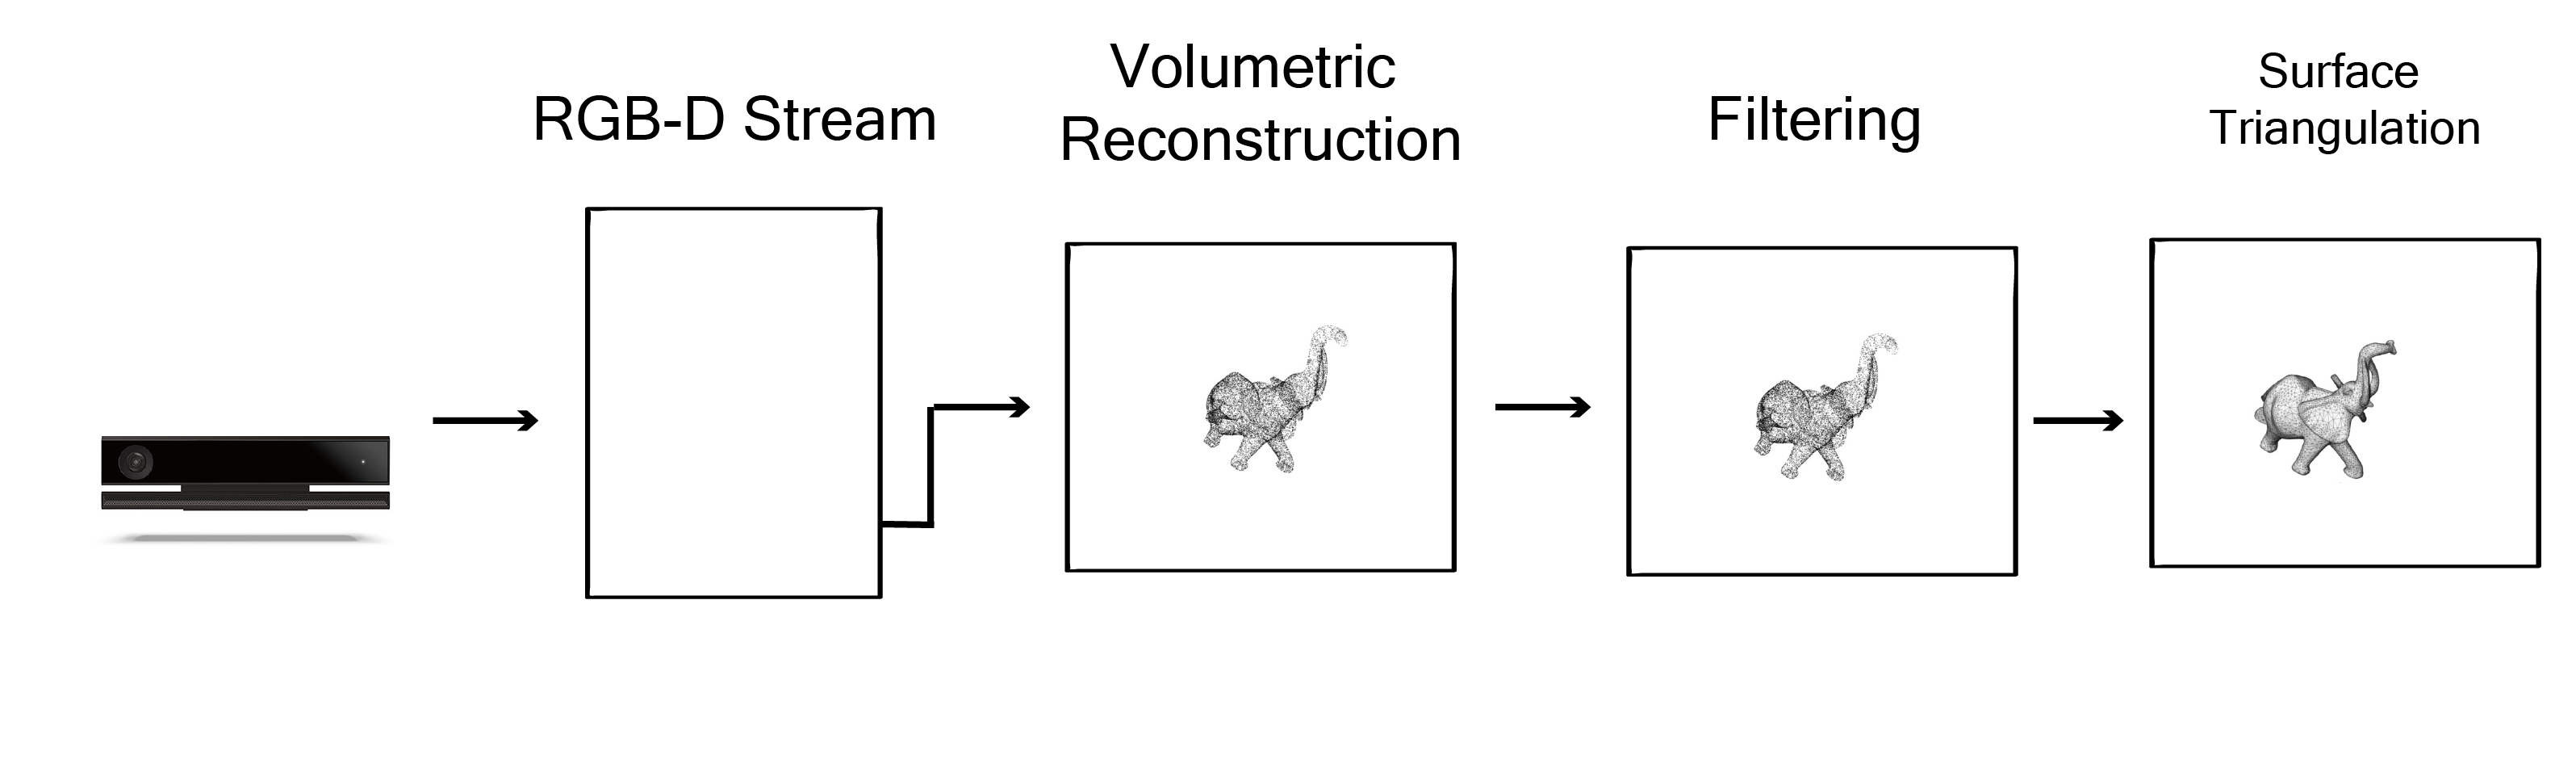
\includegraphics[scale=0.55]{pictures/pipeline_core}
    \caption{An architectural overview illustrating how raw data from the Kinect is processed to a water-tight model.}
    \label{fig:pipeline}
\end{figure}

Initially, the system continually tracks the camera pose and uses an iterative closest point ( ICP ) approach to join the live depth data into a geometrically precise 3D model of the room in real time (see \textbf{\autoref{fig:icp}}). Hereby, the camera can either be rotated around the arm or the arm itself can turn around its axis in front of the camera as long as every part is being exposed to the camera lens for a fraction of a second. Even small movements, which could be caused by a minor shake, results in a new viewport of the scene and can be used to improve the model i.e. similar to a \textit{supersampling} effect \cite{Damera-Venkata:2009:DS:1477926.1477935}.\\
\begin{figure}[ht]
    \centering
  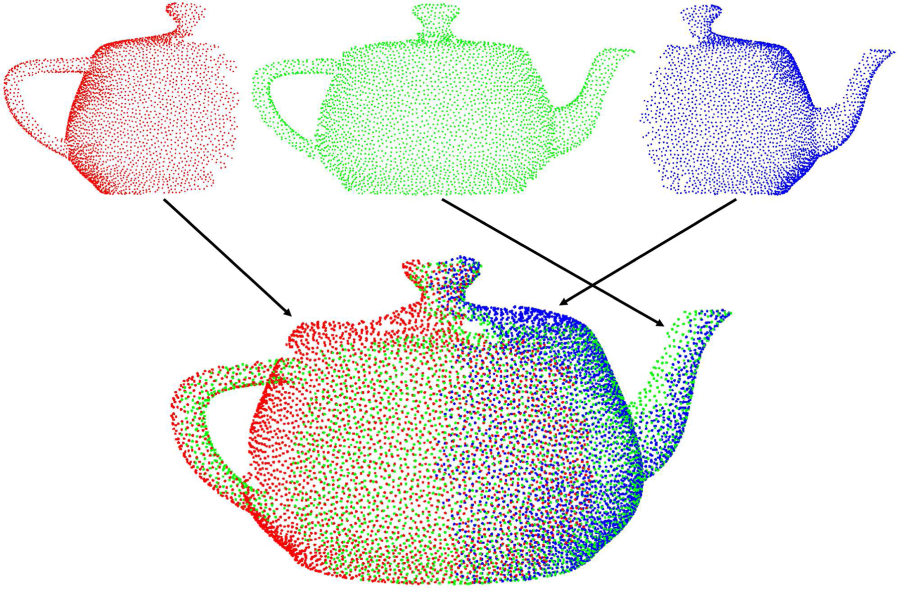
\includegraphics[scale=0.45]{pictures/icp}
    \caption{An illustration of the ICP algorithm. Multiple different views of the same object are taken iteratively to construct an overall completed model by aligning similiar features. Figure acquired from \cite{kwok2016improvements} }
    \label{fig:icp}
\end{figure}
Moving forward, several filtering methods are applied to the data set to remove background and outliers. A volumetric surface representation \cite{Curless:1996:VMB:237170.237269} is applied to the oriented point clouds which result in a continuously updated voxel grid wherein each cell stores its assumed distance to the physical surface. This surface triangulation works efficiently on the noisy data from the Kinect by filling holes and adapting to sensor motion.\\
The model then transfers to the raytracing pipeline which results in several rendered images taking physical properties into account e.g. lights and reflections. Multiple components for building an efficient acceleration structure, tree traversal and shader are asynchronously parallelized (ref sub-chapter).\\
Afterward, the user has the ability to manipulate the environment of the computated object. Each change - be it camera angle or annotations on the object - will return to the raytracing pipeline as a request for an updated image. This exchange lapses in a continuous feedback loop and will only end when the user resets the model.\\
At last, the generated drawing is extracted and the data evaluates to a coherent graph. All vertices and edges flatten from a 3D perspective into a 2D plane in SVG format (ref sub-chapter).\\
The finished shape can be further used in a postprocessing pipeline to initiate the fabrication process for a multi-touch sensor \cite{Nittala:2018:MST:3173574.3173607}.

\newpage
\pagebreak